%  -----------------------------------------------------------------------------
%  Author         : Bimalka Piyaruwan Thalagala
%  GitHub         : https://github.com/bimalka98
%  Date Created   : 11/8/2021
%  Last Modified  :
%  -----------------------------------------------------------------------------

\documentclass[a4paper,11pt]{article}%,twocolumn
\input{settings/packages}
\input{settings/page}
\input{settings/macros}
\usepackage[ framed, numbered]{matlab-prettifier}%framed,%
\usepackage{listings}
\usepackage{pythonhighlight}
\usepackage{pdfpages}

\begin{document}

\begin{titlepage}
\center % Center everything on the page

%-------------------------------------------------------------------------------------
%	HEADING SECTIONS
%------------------------------------------------------------------------------------
\textbf{\large Department of Electronic and Telecommunication Engineering}\\[0.5cm]
\textbf{\Large University of Moratuwa, Sri Lanka}\\[1cm]
\textbf{\large EN3053 - Digital Communications - I}\\[2cm]
\includegraphics[width=0.3\textwidth]{figures/uomlogo}\\[2cm]

	
%-------------------------------------------------------------------------------------
%	TITLE SECTION
%------------------------------------------------------------------------------------
\textbf{\Huge Lab Assignment}\\[0.5cm]
\textbf{\Large Eye diagrams and Equalization }\\


%----------------------------------------------------------------------------------------
%	MEMBERS SECTION
%----------------------------------------------------------------------------------------
\vfill % Fill the rest of the page with whitespace

\textbf{\large Submitted by}\\[0.5cm]
\begin{minipage}{0.2\textwidth}
	\begin{flushleft}
		{\large Thalagala B.P.}\\[4mm]
		{\large Samarasinghe P.}\\[4mm]

		
		
	\end{flushleft}
\end{minipage}
\hspace{5mm}
\begin{minipage}{0.2\textwidth}
	\begin{flushright}
		{\large 180631J }\\[4mm]
		{\large 180554B }\\[4mm]

	\end{flushright}
\end{minipage}\\[1.5cm]

%----------------------------------------------------------------------------------------
%	DATE SECTION
%----------------------------------------------------------------------------------------

\textbf{\large Submitted on}\\[0.5cm]
\textbf{\Large \today} % Date, change the \today to a set date if you want to be precise

%----------------------------------------------------------------------------------------



\end{titlepage}




\pagebreak
%%-----------------------------------------------------------------------
\includepdf[pages=-, width=\textwidth]{code/answers.pdf}



\section*{Question 4}
\subsection*{(a) The sequence of signals (waveforms) corresponding to the binary sequence}

Please note that when plotting the below figure following values were assumed for the parameters.\\

\begin{tabular}{l l}
	Bit interval ($T_b$) & 1 $s$ \\
	Symbol interval  (T) &$2 \times T_b = $  2 $s$
\end{tabular}

\begin{figure}[!h]
	\centering
	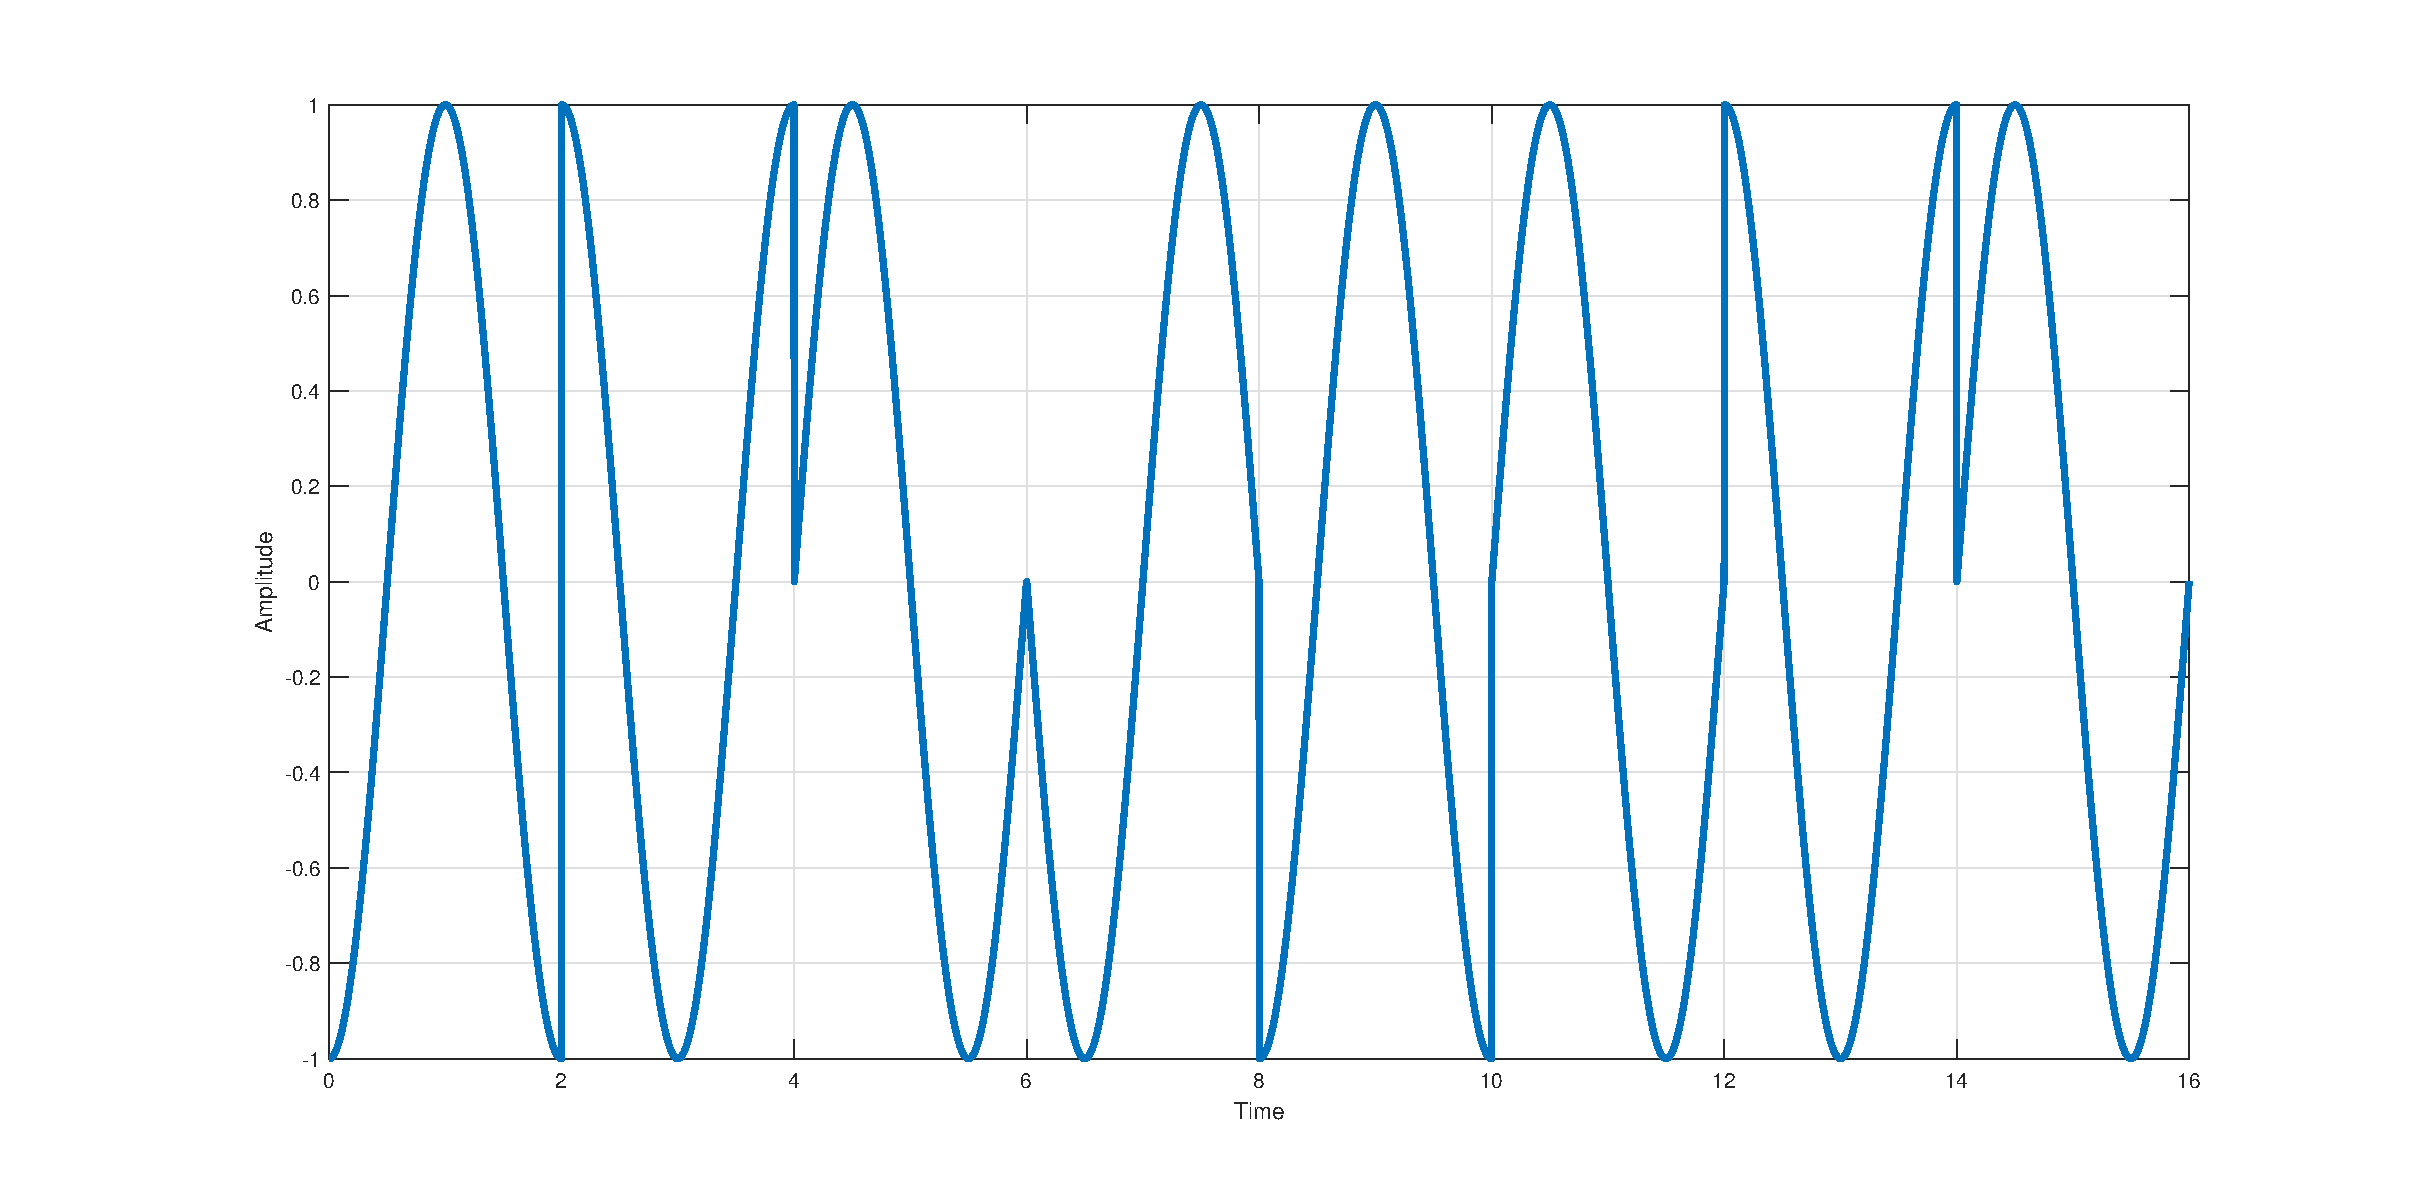
\includegraphics[scale=0.35]{figures/fig4a}
\end{figure}

\lstinputlisting[basicstyle = \mlttfamily\scriptsize , style = Matlab-editor]{code/codea.m}

\pagebreak
\subsection*{(b) The Quaternary MSK phase trajectory}
Please note that when plotting the below figure following values were assumed for the parameters.\\

\begin{tabular}{l l}
	Bit interval ($T_b$) & 1 $s$ \\
	Symbol interval  (T) &$2 \times T_b = $  2 $s$
\end{tabular}

\begin{figure}[!h]
	\centering
	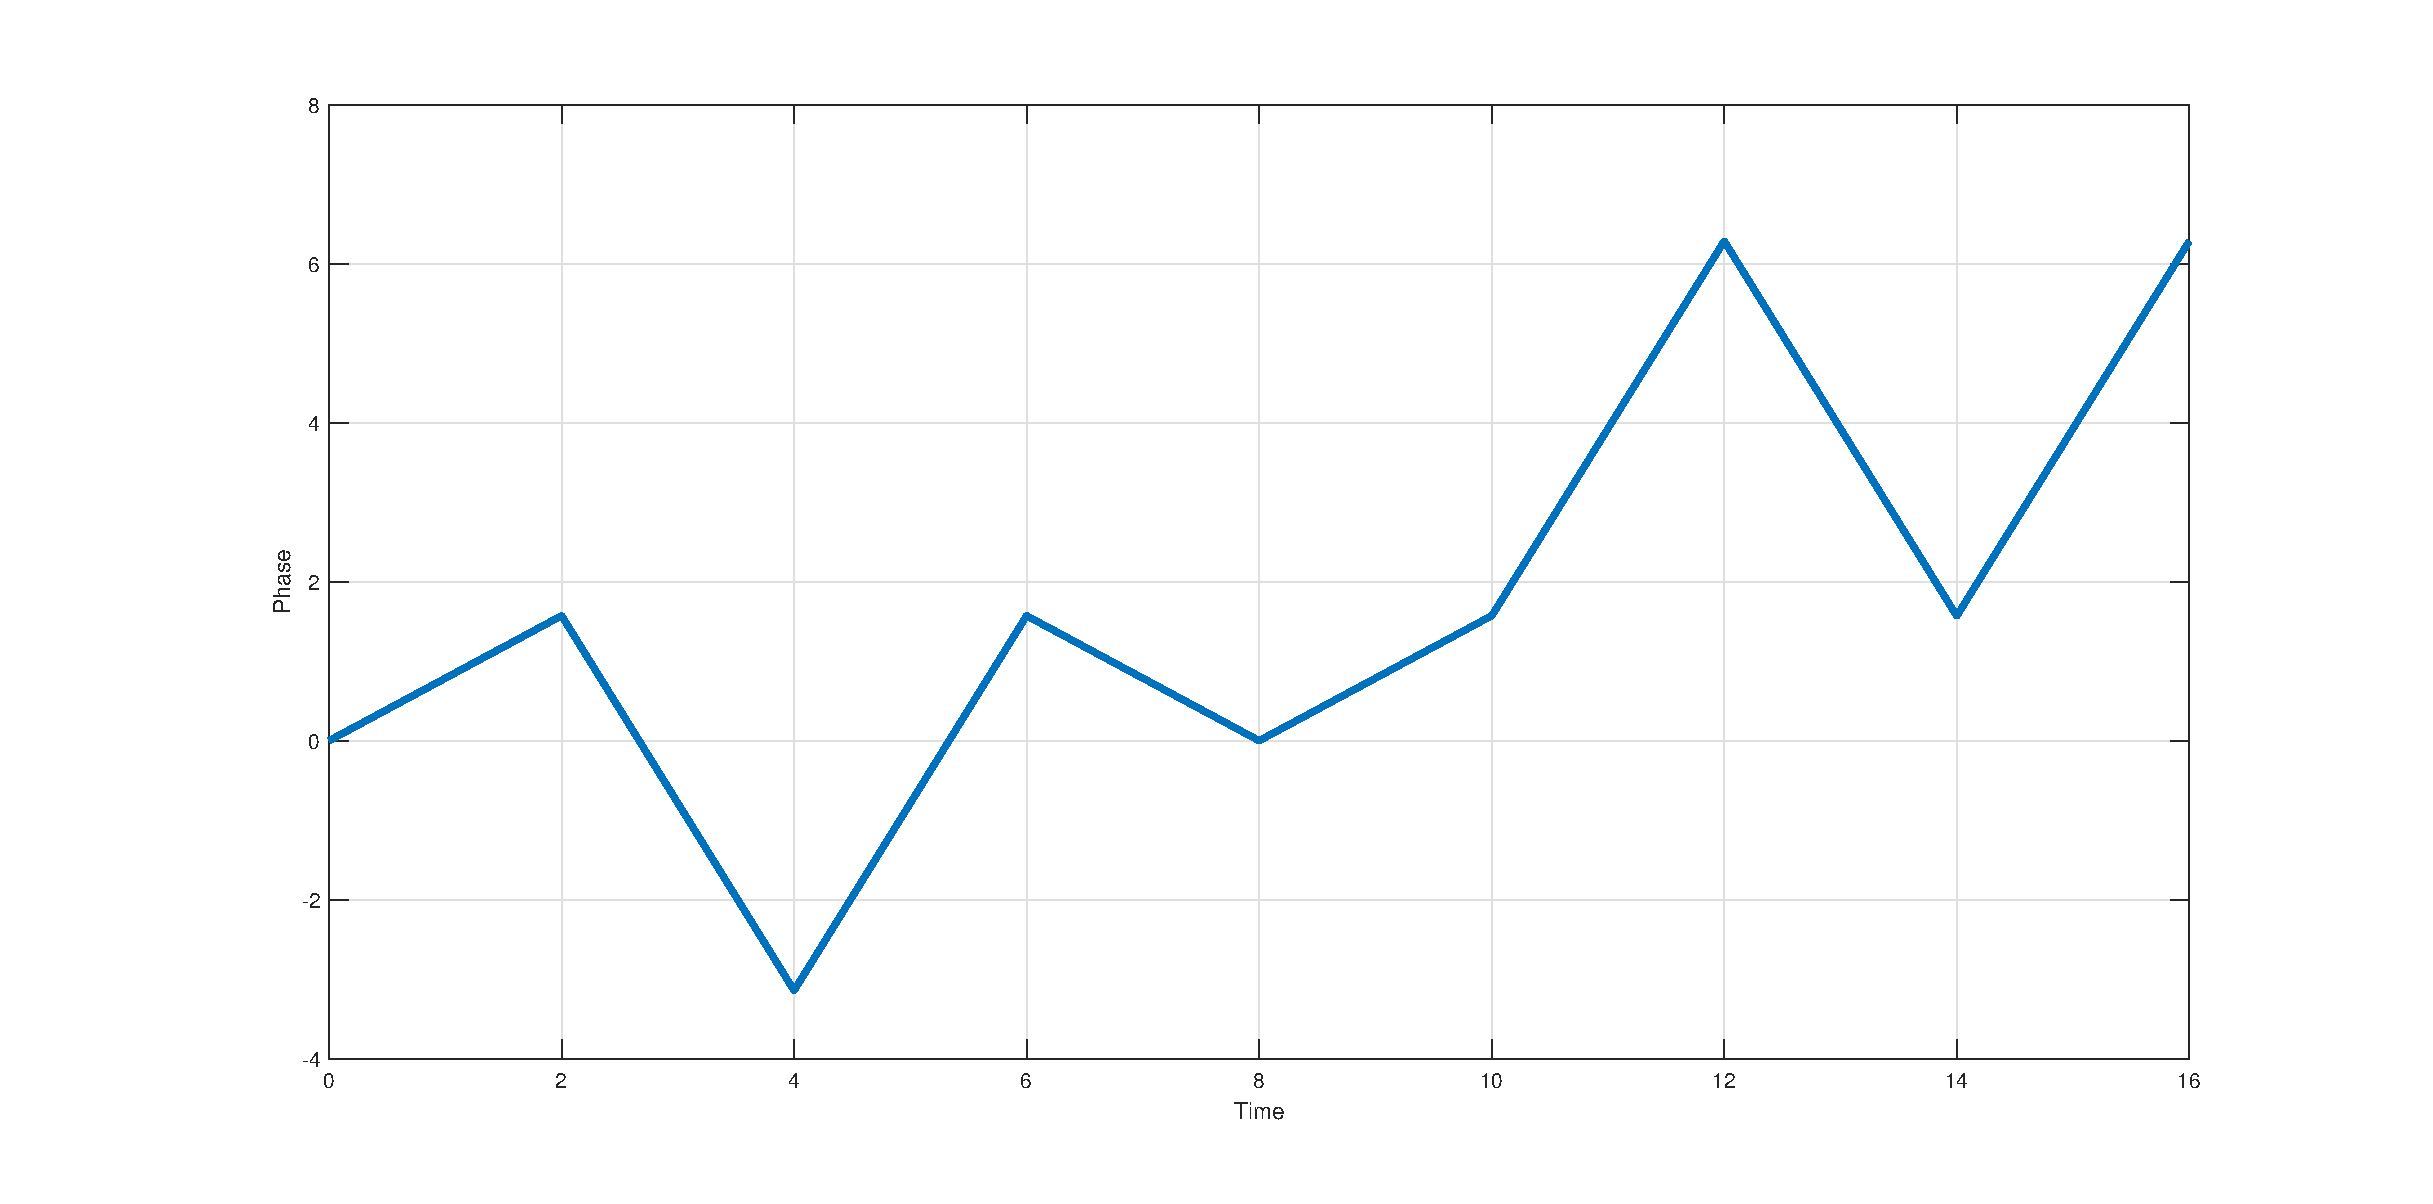
\includegraphics[scale=0.35]{figures/fig4b}
\end{figure}

\lstinputlisting[basicstyle = \mlttfamily\scriptsize , style = Matlab-editor]{code/codeb.m}

\pagebreak
\subsection*{(c) The Quaternary MSK waveform corresponding to the binary sequence}
Please note that when plotting the below figure following values were assumed for the parameters.\\

\begin{tabular}{l l}
	Bit interval ($T_b$) & 1 $s$ \\
	Symbol interval  (T) &$2 \times T_b = $  2 $s$
\end{tabular}

\begin{figure}[!h]
	\centering
	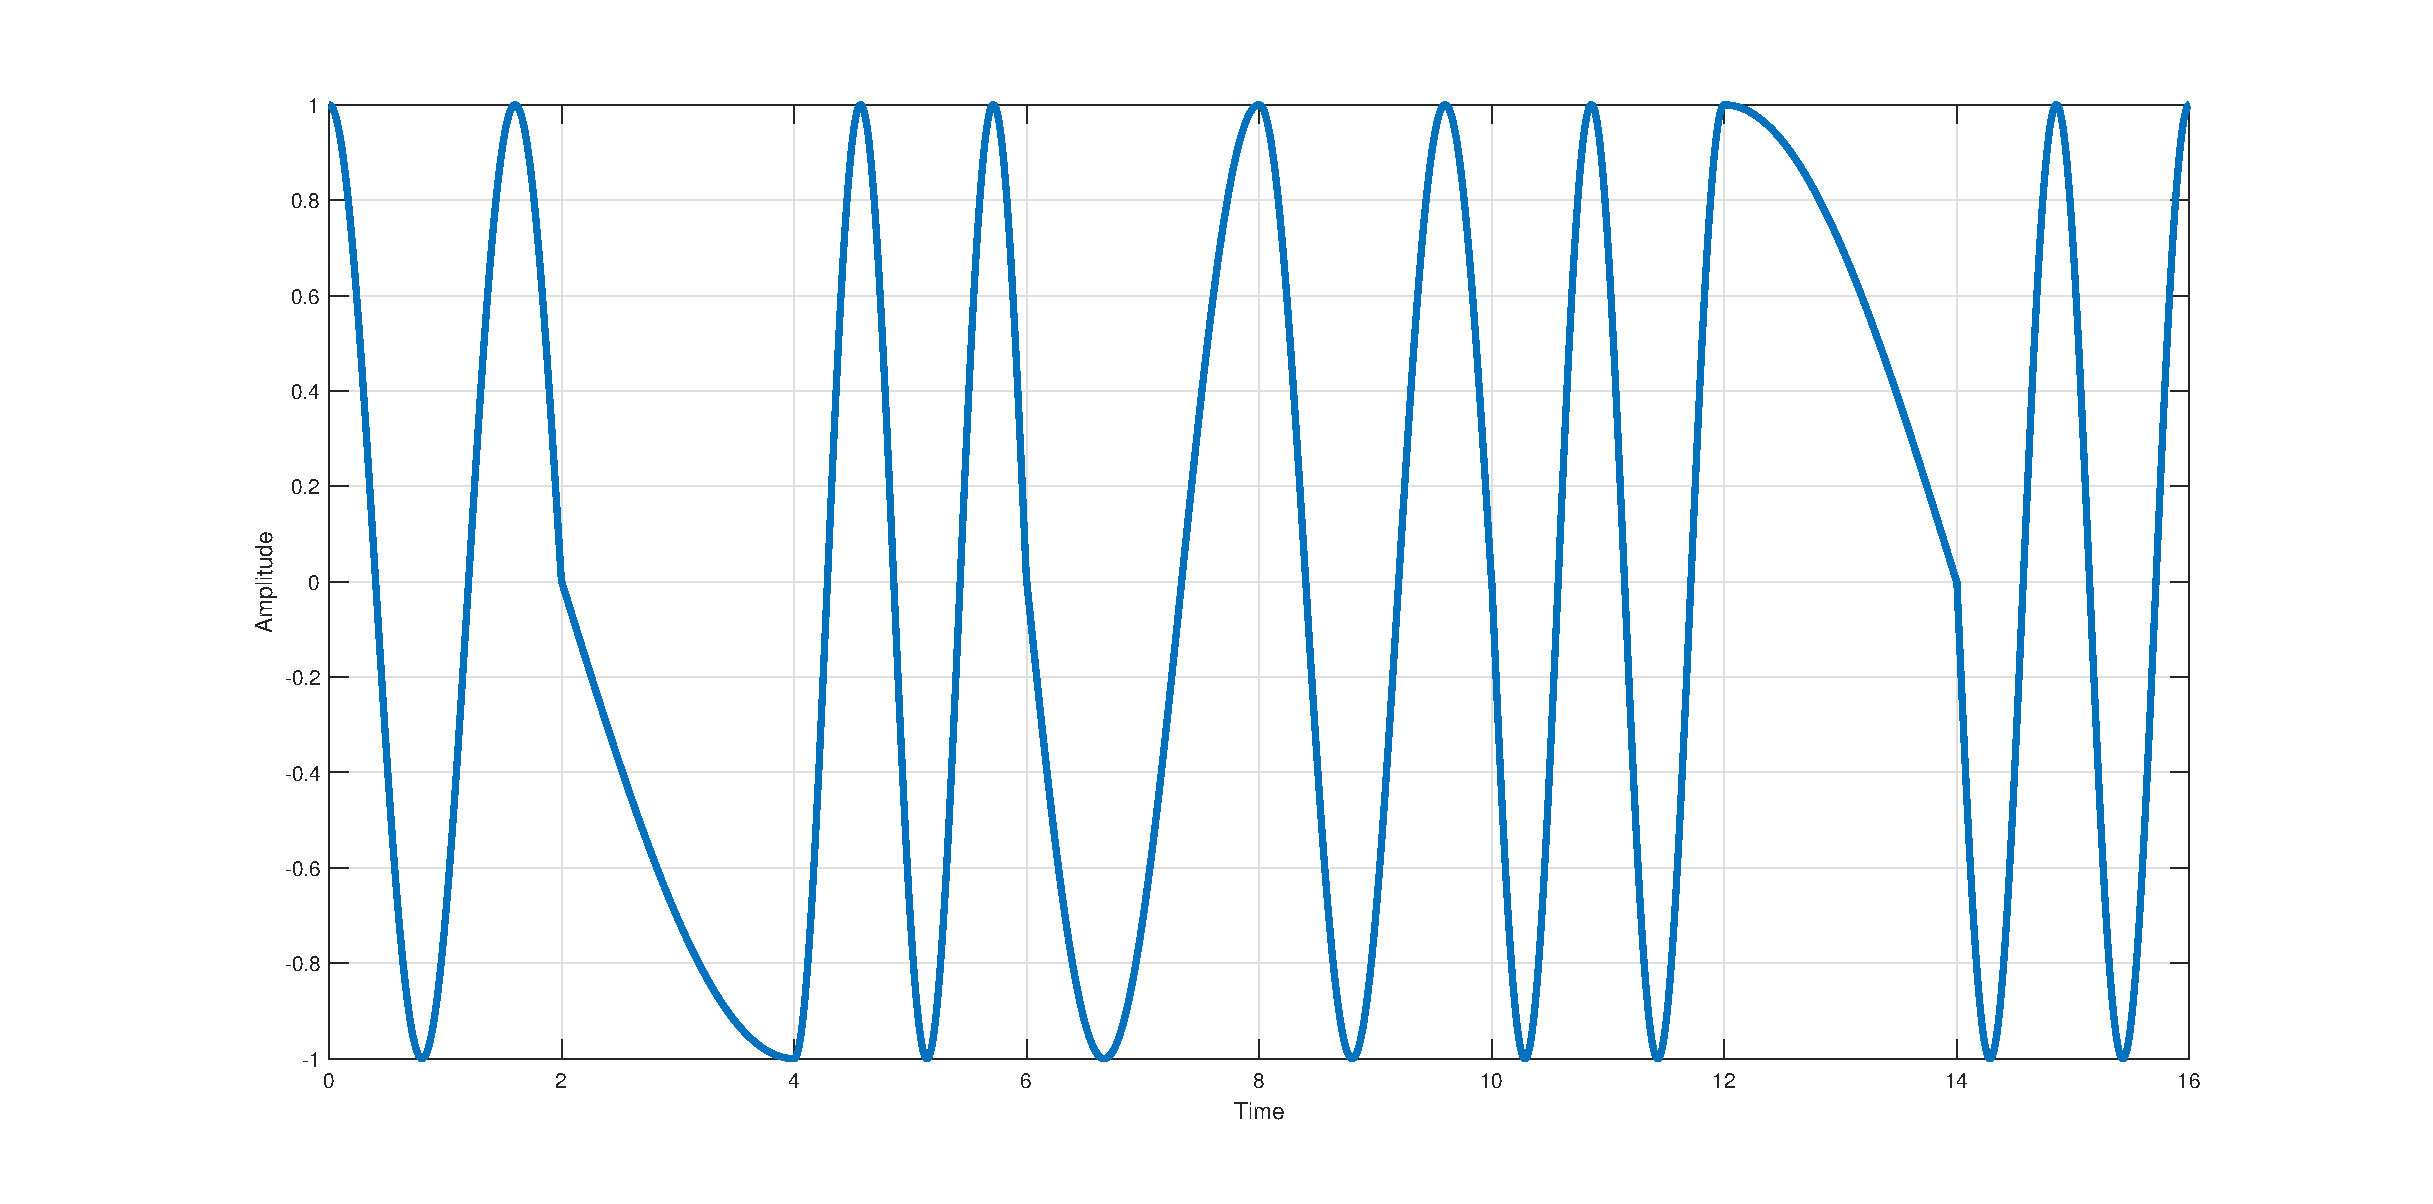
\includegraphics[scale=0.35]{figures/fig4c}
\end{figure}

\lstinputlisting[basicstyle = \mlttfamily\scriptsize , style = Matlab-editor]{code/codec.m}
%---------------------------------------------------------------------------
\end{document}
